\documentclass[12pt,letterpaper]{article}
\usepackage[utf8]{inputenc}
\usepackage{amsmath,amssymb,fullpage,graphicx}
\usepackage{subfigure}
\let\hat\widehat
\let\tilde\widetilde


\author{Nan Tang \\ 1662478}
	%% your name
\title{STAT 403 Spring 2018\\HW07}
	%% title of this document
\begin{document}
\maketitle
	%% make the title and author

\section*{Q1}
\subsection*{Q1-a}
\begin{verbatim}
petal_wdt_ln <- lm(Petal.Width~Sepal.Length + Sepal.Width + Petal.Length, data=iris)
petal_wdt_ln$coefficients

 (Intercept) Sepal.Length  Sepal.Width Petal.Length 
  -0.2403074   -0.2072661    0.2228285    0.5240831 
\end{verbatim}

\noindent For fitted linear model, the intercept is -0.2403074, slope of sepal length is -0.2072661, slope of sepal width is  0.2228285, and slope of petal length is  0.5240831.

\subsection*{Q1-b}
\begin{verbatim}
# empirical bootstrap
cal_var <- function(dt, col_num) {
  result <- rep(NA, col_num)
  for (ii in 1:col_num) {
    result[ii] <- var(dt[, ii])
  }
  return(result)
}

n <- nrow(iris)
B <- 10000
reg_ep_bt <- matrix(NA, nrow=B, ncol=4)
for (ii in 1:B) {
  sp_index <- sample(n, n, replace=T)
  sp_dt <- iris[sp_index,]
  sp_ln <- lm(Petal.Width~Sepal.Length + Sepal.Width + Petal.Length, data=sp_dt)
  reg_ep_bt[ii,] <- sp_ln$coefficients 
}
var_ep_bt <- cal_var(reg_ep_bt, 4)

# residual bootstrap
y_predict <- predict(petal_wdt_ln)
reg_resid_bt <- matrix(NA, nrow=B, ncol=4)
for (ii in 1:B) {
  sp_index <- sample(n, n, replace=T)
  sp_y <- petal_wdt_ln$residuals[sp_index] + y_predict
  sp_dt <- data.frame(Sepal.Length=iris$Sepal.Length, Sepal.Width=iris$Sepal.Width, 
                      Petal.Length=iris$Petal.Length, Petal.Width=sp_y)
  sp_ln <- lm(Petal.Width~Sepal.Length + Sepal.Width + Petal.Length, data=sp_dt)
  reg_resid_bt[ii,] <- sp_ln$coefficients
}
var_resid_bt <- cal_var(reg_resid_bt, 4)

# wild bootstrap
reg_wild_bt <- matrix(NA, nrow=B, ncol=4)
for (ii in 1:B) {
  sp_y <- rnorm(n, sd=abs(petal_wdt_ln$residuals)) + y_predict
  sp_dt <- data.frame(Sepal.Length=iris$Sepal.Length, Sepal.Width=iris$Sepal.Width, 
                      Petal.Length=iris$Petal.Length, Petal.Width=sp_y)
  sp_ln <- lm(Petal.Width~Sepal.Length + Sepal.Width + Petal.Length, data=sp_dt)
  reg_wild_bt[ii,] <- sp_ln$coefficients
}
var_wild_bt <- cal_var(reg_wild_bt, 4)

var_result <- rbind(var_ep_bt, var_resid_bt, var_wild_bt)
rownames(var_result) <- c('Empirical bt', 'Residual bt', 'Wild bt')
colnames(var_result) <- c('Intercept', 'Sepal.Length', 'Sepal.Width', 'Petal.Length')

> var_result
              Intercept Sepal.Length Sepal.Width Petal.Length
Empirical bt 0.03726415  0.002452046 0.002268225 0.0006252015
Residual bt  0.03127332  0.002187685 0.002343256 0.0005825280
Wild bt      0.03501799  0.002387478 0.002106485 0.0006052753
\end{verbatim}

\newpage
\subsection*{Q1-c}
\begin{verbatim}
library(plotrix)
p <- multhist(list(reg_ep_bt[,1], reg_resid_bt[,1], reg_wild_bt[,1]), probability=T,
              main='Histograms of Bootstrap Intercept', xlab='Bootstrap Intercept')
legend('topright', c('Empirical', 'Residual', 'Wild'), 
       col=c('gray30', 'gray55', 'gray80'),lwd=5, cex = 0.75)
\end{verbatim}

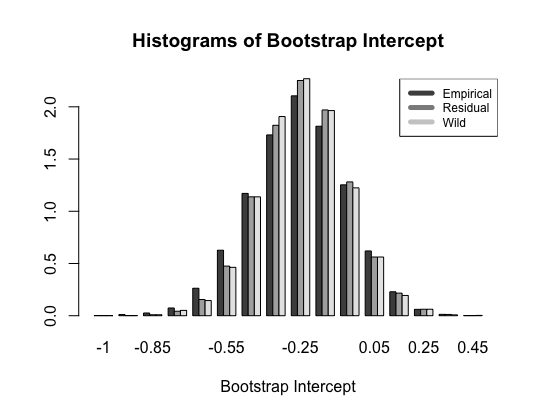
\includegraphics[width=150mm]{q1-c-2.png}

\newpage
\section*{Q2-a}
\begin{verbatim}
admission_dt <- read.csv('binary.csv', header =T)
binom_logistic <- glm(admit~gpa + gre, data=admission_dt, family='binomial')
B <- 10000
n <- nrow(admission_dt)

par_bt_slope <- rep(NA, B)
for (ii in 1:B) {
  sp_admit <- rbinom(n, size=1, prob=predict(binom_logistic, type='response'))
  sp_dt <- data.frame(admit=sp_admit, gpa=admission_dt$gpa, gre=admission_dt$gre)
  sp_logistic <- glm(admit~gpa + gre, data=sp_dt, family='binomial')
  par_bt_slope[ii] <- sp_logistic$coefficients[2]
}

> quantile(par_bt_slope, 0.05)
       5% 
0.2258055 
> quantile(par_bt_slope, 0.95)
     95% 
1.292753 
\end{verbatim}

\noindent $90 \%$ CI for slope of gpa is $[0.2258055, 1.292753 ]$.

\subsection*{Q2-b}
\begin{verbatim}
par_bt_three <- matrix(NA, nrow=B, ncol=3)
for (ii in 1:B) {
  sp_admit <- rbinom(n, size=1, prob=predict(binom_logistic, type='response'))
  sp_dt <- data.frame(admit=sp_admit, gpa=admission_dt$gpa, gre=admission_dt$gre)
  sp_logistic <- glm(admit~gpa + gre, data=sp_dt, family='binomial')
  par_bt_three[ii,] <- sp_logistic$coefficients
}
par_bt_sd <- c(sd(par_bt_three[,1]), sd(par_bt_three[,2]), sd(par_bt_three[,3]))

ep_bt_three <- matrix(NA, nrow=B, ncol=3)
for (ii in 1:B) {
  sp_index <- sample(n, n, replace=T)
  sp_dt <- admission_dt[sp_index, ]
  sp_logistic <- glm(admit~gpa + gre, data=sp_dt, family='binomial')
  ep_bt_three[ii,] <- sp_logistic$coefficients
}
head(ep_bt_three)
ep_bt_sd <- c(sd(ep_bt_three[,1]), sd(ep_bt_three[,2]), sd(ep_bt_three[,3]))

result_sd <- rbind(summary(binom_logistic)$coefficients[,2], par_bt_sd, ep_bt_sd)
colnames(result_sd) <- c('Intercept', 'gpa', 'gre')
rownames(result_sd) <- c('original', 'parametric bt', 'empirical bt')

> result_sd
              Intercept       gpa         gre
original       1.075093 0.3195856 0.001057491
parametric bt  1.092944 0.3231437 0.001070655
empirical bt   1.085661 0.3398939 0.001090929
\end{verbatim}

\subsection*{Q2-c}
\noindent Use empirical bootstrap to estimate probability that John will be admitted.
\begin{verbatim}
prob_bt <- rep(NA, B)
for (ii in 1:B) {
  sp_index <- sample(n, n, replace=T)
  sp_dt <- admission_dt[sp_index,]
  sp_logis <- glm(admit~gpa + gre, data=sp_dt, family='binomial')
  prob_bt[ii] <- predict(sp_logis, type='response', data.frame(gpa=3.7, gre=500))
}
lower_bd <- quantile(prob_bt, 0.05)
upper_bd <- quantile(prob_bt, 0.95)

> lower_bd
       5% 
0.2387916 
> upper_bd
      95% 
0.3782043 
\end{verbatim}

\noindent The $90 \%$ CI of $\lambda = P(admit=1, gpa=3.7, gre=500)$ is $[0.2387916 , 0.3782043]$.

\newpage
\subsection*{Q2-d}
\noindent Let $P_1$ denotes probability of John being admitted, and $P_2$ denotes probability of Sam being admitted. 

\noindent Let $\delta$ denotes $(P_1 - P_2)$

\noindent First bootstrap 10000 simulations for $P_1$ and $P_2$ to get standard deviation of $\delta$.
\begin{verbatim}
probs_bt <- matrix(NA, nrow=B, ncol=2)
for (ii in 1:B) {
  sp_index <- sample(n, n, replace=T)
  sp_dt <- admission_dt[sp_index,]
  sp_logis <- glm(admit~gpa + gre, data=sp_dt, family='binomial')
  probs_bt[ii, 1] <- predict(sp_logis, type='response', data.frame(gpa=2.3, gre=700))
  probs_bt[ii, 2] <- predict(sp_logis, type='response', data.frame(gpa=3.9, gre=670))
}
delta <- probs_bt[,1] - probs_bt[,2]
hist(delta)
delta_sd <- sd(delta)

> delta_sd
[1] 0.1004981
\end{verbatim}

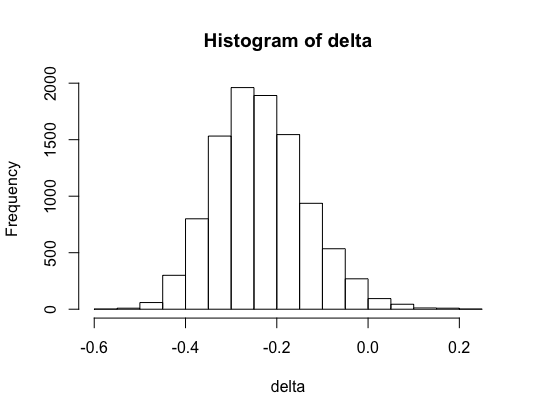
\includegraphics[scale=0.7]{q2-d.png}

\noindent The distribution of $delta$ is approximately normal.  \\

\begin{verbatim}
observed_prob1 <- predict(binom_logistic, type='response', data.frame(gpa=2.3, gre=700))
observed_prob2 <- predict(binom_logistic, type='response', data.frame(gpa=3.9, gre=670))
observed_delta <- observed_prob1 - observed_prob2

> observed_delta
-0.2401996 

p_value <- 2 * pnorm(observed_delta, sd=delta_sd)
> p_value
0.01684422 

\end{verbatim}

\noindent Observed probability difference is $-0.24$ with p-value equals to $0.01684422$. \\

\noindent $p-value < 0.1$, thereby we may reject the null hypothesis under test size $0.1$.



%%% do not touch anything below
\end{document}
